% !TeX spellcheck = pt_BR

%%%%%%%%%%%%%%%%%%%%%%%%%%%%%%%%%%%%%%%%%%%%%%%
% Modelo adaptado do template original de
% Ted Pavlic (http://www.tedpavlic.com)
% Todos os créditos a ele.
%
% Na versão atual, o que foi modificado
% do original:
% Ajusta a numeração das questões e
% passa para português.
% Além de separar as configurações
% em um arquivo .cls separado.
%
% Crédito ao Roberto por ter feito
% a maior parte do trabalho de passar
% para o português e fazer outros
% ajustes para a versão atual deste template.
%%%%%%%%%%%%%%%%%%%%%%%%%%%%%%%%%%%%%%%%%%%%%%%


%----------------------------------------------------------------------------------------
%	PACKAGES E OUTRAS CONFIGURAÇÕES
%----------------------------------------------------------------------------------------

\documentclass{homeworkclass}

\usepackage{animate}


\usepackage{myMacros}


\hmwkTitle{Lista\ de\ Exercícios \#2}
\hmwkDueDate{Terça,\ 23\ de\ Julho,\ 2019}
\hmwkClass{Elementos de Processamento de 	Sinais}
\hmwkClassTime{Segundas e Quartas: 08:00--10:00}
\hmwkClassInstructor{Prof.\ Sergio Lima Netto}
\hmwkAuthorName{Vinicius Mesquita de Pinho}
\hmwkAuthorShortName{Vinicius Mesquita}

\begin{document}

\maketitle

%----------------------------------------------------------------------------------------
%	SUMÁRIO
%----------------------------------------------------------------------------------------

%\setcounter{tocdepth}{1} % Uncomment this line if you don't want subsections listed in the ToC

\clearpage
\newpage
%\tableofcontents
%\newpage

%----------------------------------------------------------------------------------------
%	QUESTÃO 1
%----------------------------------------------------------------------------------------

% To have just one problem per page, simply put a \clearpage after each problem



\begin{homeworkProblem}
Para esta questão, devemos executar a síntese de um filtro de resposta ao impulso finita (FIR, do inglês \textit{finite impulse response}) pelo método denominado \textit{frequency sampling}. 

\begin{homeworkSection}[FIR fase não linear]

\paragraph{} Para o caso em que esperamos ver o nosso filtro FIR com fase não linear, sua resposta ao impulso não irá entrar em nenhum dos 4 casos de simetria (ou anti-simetria) que fazem sua resposta em frequência ter fase linear. 


\paragraph{}Vamos começar com a resposta em frequência ideal do nosso filtro. A  Figura~\ref{fig:ideal_nl} mostra sua resposta em magnitude. 

\begin{figure}[!ht]
	\centering
	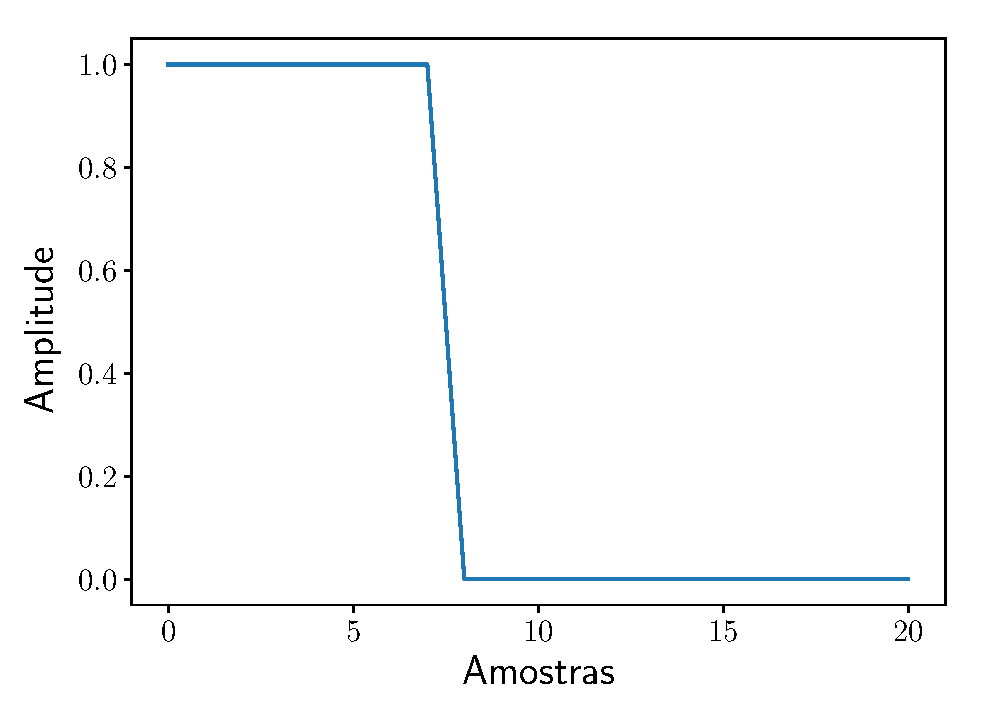
\includegraphics[width=0.5\linewidth]{figs/ideal_nl}
	\caption{Resposta em magnitude do filtro desejado.}
	\label{fig:ideal_nl}
\end{figure}

\paragraph{}O segundo passo é amostrar a nossa resposta em frequência, o resultado é apresentado na Figura~\ref{fig:ideal_amostrado_nl}.

\begin{figure}[!ht]
	\centering
	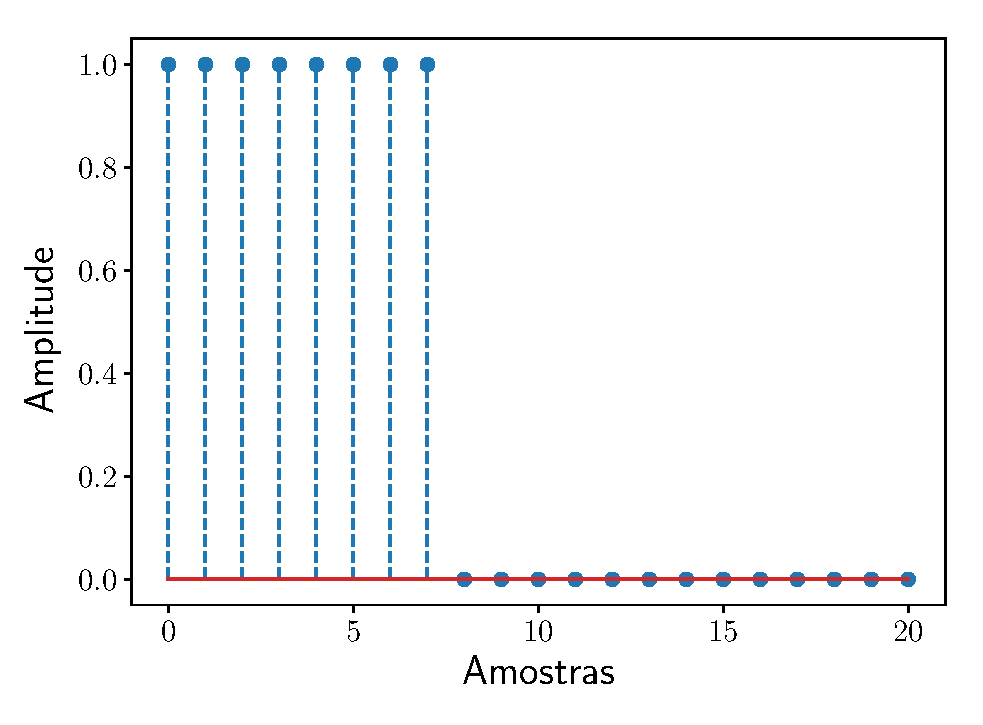
\includegraphics[width=0.5\linewidth]{figs/ideal_amostrado_nl}
	\caption{Resposta em magnitude amostrada do filtro desejado.}
	\label{fig:ideal_amostrado_nl}
\end{figure}

O que fizemos é calcular a IDFT da resposta em magnitude amostrada, e aí teremos a resposta impulso desejada. A Figura~\ref{fig:freq_nl} mostra a resposta em magnitude (em azul) e a fase (em verde) do filtro calculado a partir da estratégia de amostrar o domínio da frequência.
\begin{figure}[!ht]
	\centering
	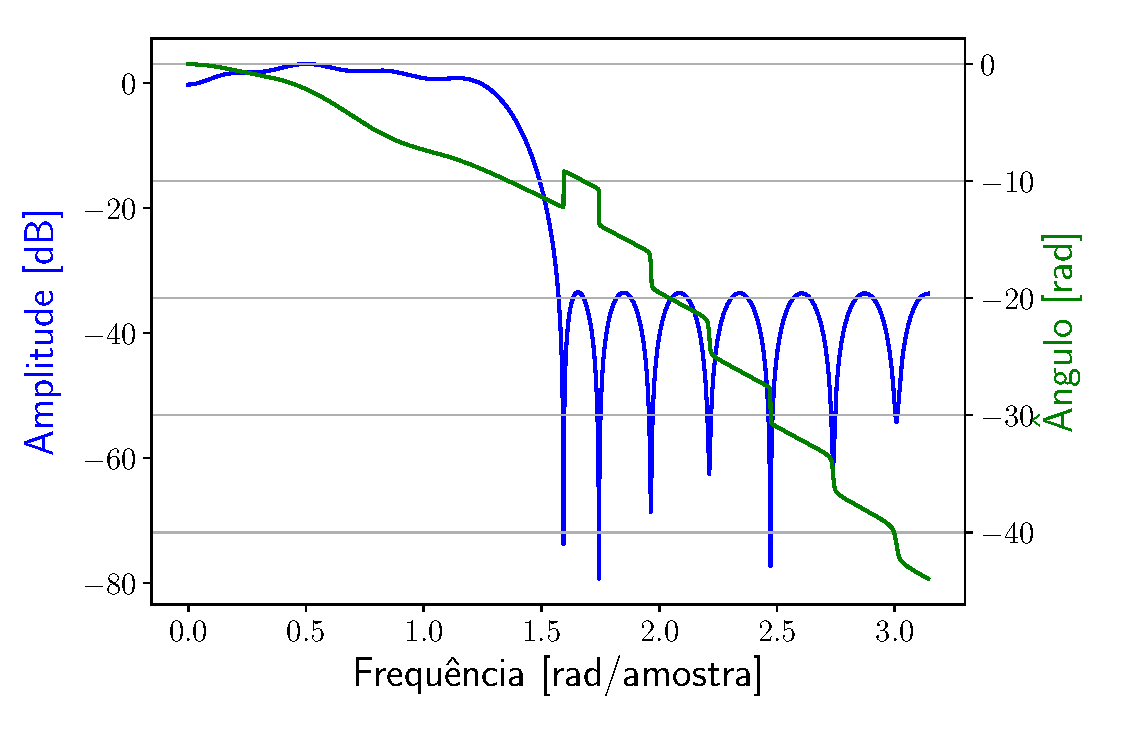
\includegraphics[width=0.6\linewidth]{figs/freq_nl}
	\caption{Resposta em frequência do filtro desejado.}
	\label{fig:freq_nl}
\end{figure}



\end{homeworkSection}


\begin{homeworkSection}[FIR fase linear]

Agora para o caso em que desejamos fase linear, nossa resposta ao impulso terá simetria.

\paragraph{}Vamos começar com a resposta em frequência ideal do nosso filtro. A Figura~\ref{fig:ideal} mostra a resposta em magnitude do filtro ideal.

\begin{figure}[!ht]
	\centering
	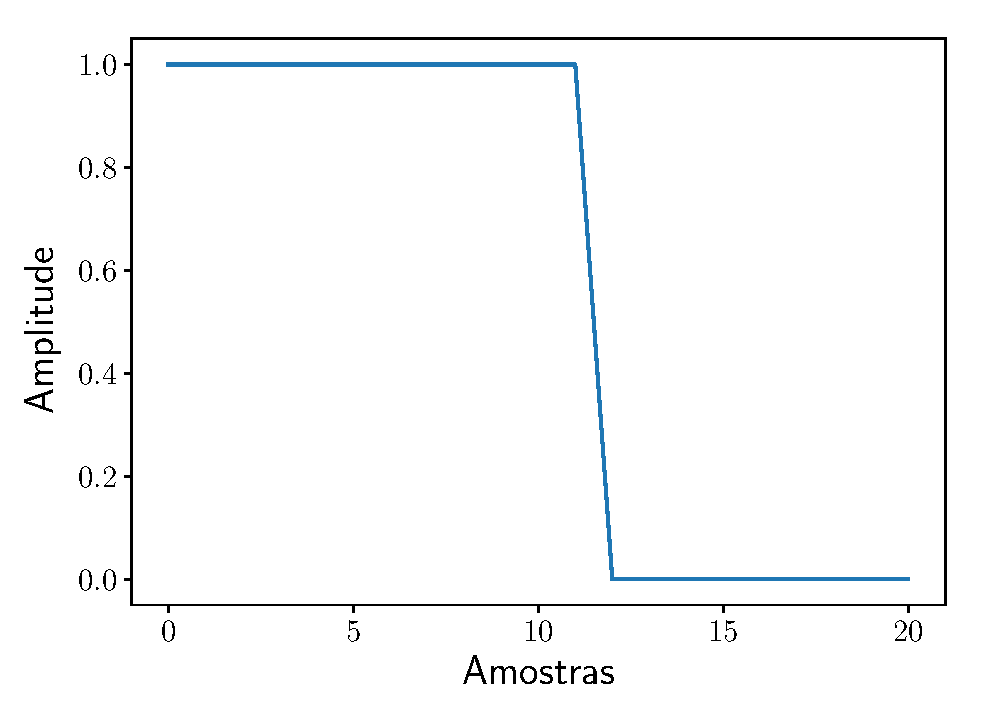
\includegraphics[width=0.6\linewidth]{figs/ideal}
	\caption{Resposta em frequência do filtro desejado.}
	\label{fig:ideal}
\end{figure}

\paragraph{}O segundo passo é amostrar a nossa resposta em frequência, o resultado é apresentado na Figura~\ref{fig:ideal_amostrado}.

\begin{figure}[!ht]
	\centering
	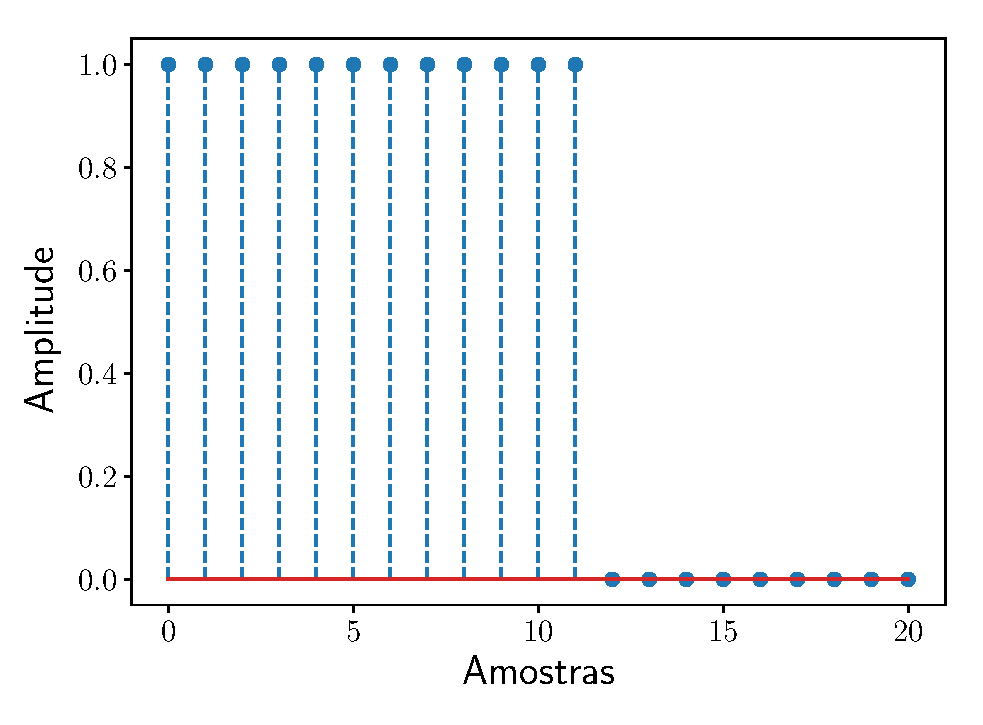
\includegraphics[width=0.6\linewidth]{figs/ideal_amostrado}
	\caption{Resposta em frequência do filtro desejado.}
	\label{fig:ideal_amostrado}
\end{figure}

\paragraph{}O sinal é flipado e concatenado com ele mesmo, de modo que o que vemos na Figura~\ref{fig:ideal_amostrado_nl} é na verdade parte da resposta em frequência.


\paragraph{}Segundo a teoria apresentada no livro-texto, para $M$ par e resposta ao impulso simétrica, a fase $\theta(k)$ e a amplitude $A(k)$ devem ser:
\begin{align*}
	\theta(k) &= - \frac{- \pi k M}{M+1}, \, \, \textrm{para} \, \, 1 \leq k \leq M, \\
	A(k) &= A(M-k+1), \, \, \textrm{para} \, \, 1 \leq k \leq \frac{M}{2}.
\end{align*}
Entõa a response ao impulso é dada por 
\begin{equation}
h(n) = \frac{1}{M+1}\left[A(0) + 2\sum_{k=1}^{M/2}(-1)^{k}A(k)\cos\frac{\pi k(1+ 2n)}{M+1}\right]
\end{equation}

Realizando os calculos, calculamos a resposta ao impulso que é representada na Figura~\ref{fig:freq} por sua resposta em magnitude (em azul) e sua fase (em verde). Podemos ver que a mesma tem fase linear na banda passante.

\begin{figure}[!ht]
	\centering
	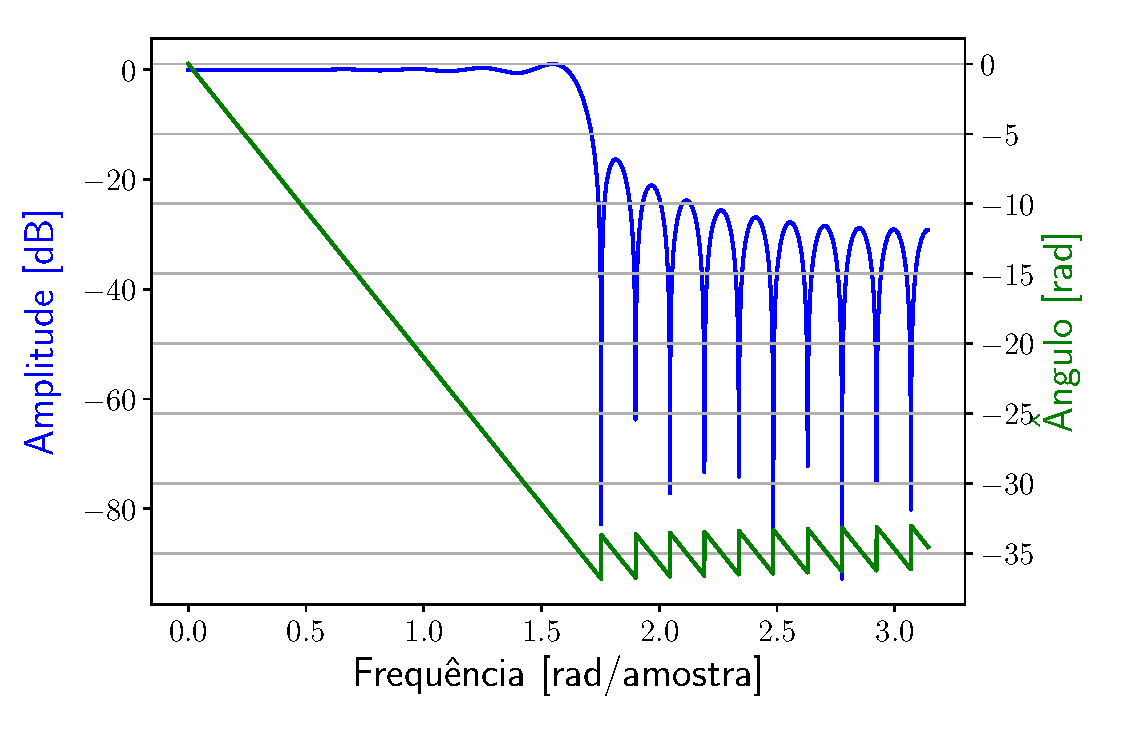
\includegraphics[width=0.6\linewidth]{figs/freq}
	\caption{Resposta em frequência do filtro desejado.}
	\label{fig:freq}
\end{figure}

\end{homeworkSection}
\end{homeworkProblem}

\end{document}